\documentclass{beamer}
\usepackage{physics}
\usepackage{amsmath}
\usepackage{tikz}
\usepackage{mathdots}
\usepackage{yhmath}
\usepackage{cancel}
\usepackage{color}
\usepackage{siunitx}
\usepackage{array}
\usepackage{multirow}
\usepackage{amssymb}
\usepackage{textcomp, gensymb}
\usepackage{tabularx}
\usepackage{extarrows}
\usepackage{booktabs}
\usetikzlibrary{fadings}
\usetikzlibrary{patterns}
\usetikzlibrary{shadows.blur}
\usetikzlibrary{shapes}
\usepackage{listings}
\usepackage{hyperref}

%Information to be included in the title page:
\title{Numerical bootstrap}
\author{Jinyuan Wu}
\institute{Department of Physics, Fudan University}
\date{2021}

\usetheme{Madrid}

\newcommand{\concept}[1]{\textbf{#1}}

\begin{document}

\frame{\titlepage}

\begin{frame}
\frametitle{Introduction}

\textbf{What's bootstrap}

\begin{itemize}
    \item A quantum theory = expectations of all Hermitian operators; 
    Hamiltonian/Lagrangian $\Leftrightarrow$ ``probability distribution''
    \item Constraint on the system $\Rightarrow$ relation between different $\expval{O}$'s (``\concept{data}'');
    independent $\expval{O}$'s $\Leftrightarrow$ parameters in the model
    \item Inequality constraint (e.g. positivity of $\expval{O^\dagger O}$) $\Rightarrow$ allowed 
    range of $\expval{O}$'s
    \item Solving a class of problems without mentioning explicitly the wave function/path integral: 
    hence the name \emph{bootstrap}
\end{itemize}

\vspace{1em}

\end{frame}

\begin{frame}
\frametitle{Example: conformal bootstrap}

\begin{itemize}
    \item The most famous example: \concept{conformal bootstrap}
    \item Constraints: (spinless) two-point function 
    \begin{equation}
        \expval*{\mathcal{O}(x) \mathcal{O}(y)} = \frac{1}{\abs*{x - y}^{2 \Delta_\mathcal{O}}},
    \end{equation}
    three-point function 
    \begin{equation}
        \begin{aligned}
            &\quad \langle\mathcal{A}(x) \mathcal{B}(y) \mathcal{C}(z)\rangle \\
            &= \frac{f_{\mathcal{A B C}}}{|x-y|^{\Delta \mathcal{A}+\Delta_{\mathcal{B}}-\Delta_{\mathcal{C}}}|y-z|^{\Delta_{\mathcal{B}}+\Delta_{\mathcal{C}}-\Delta \mathcal{A}}|z-x|^{\Delta_{\mathcal{C}}+\Delta_{\mathcal{A}}-\Delta_{\mathcal{B}}}}
        \end{aligned}
    \end{equation}
    Higher order correlation functions: OPEs. 
    \item Independent parameters: $\{\Delta_{\mathcal{O}}, l_{\mathcal{O}}, f_{\mathcal{A} \mathcal{B} \mathcal{C}}\}$
    \item Inequality constraints (self-consistent conditions): determining the range of parameters
\end{itemize}

\end{frame}

\begin{frame}
\frametitle{Example: conformal bootstrap}

\begin{itemize}
    \item Example of conformal bootstrap: verify whether the critical point of 3D Ising model 
    is a CFT and its position in the allowed region\footnote{arXiv \href{https://arxiv.org/abs/1203.6064}{1203.6064}}
    \item Physical picture tells us there are two degrees of freedom: energy density $\epsilon$, spin field $\sigma$
    \item Below is Fig.~3 in the paper: comparing critical exponents of 3D Ising model, and the allowed range from conformal bootstrap
\end{itemize}

\begin{center}
    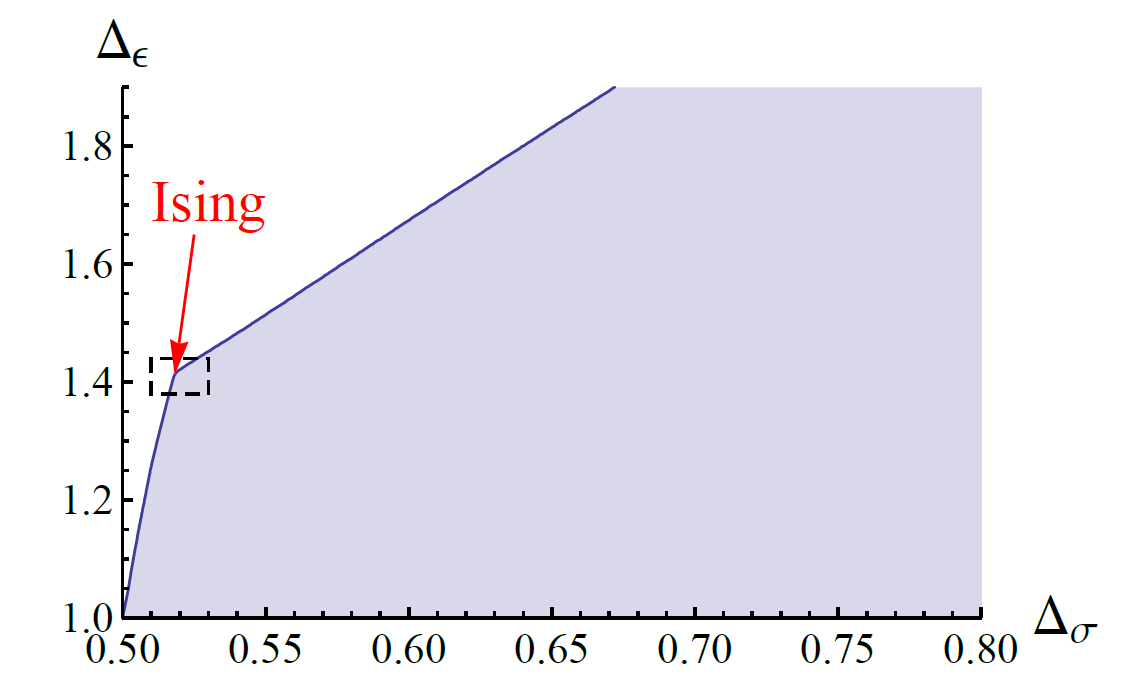
\includegraphics[width=0.5\textwidth]{3d-ising-cft-bootstrap-range.PNG}
\end{center}

\end{frame}

\begin{frame}
\frametitle{Bootstrap for generic systems}

\textbf{How to perform bootstrap for a generic system?}    

\begin{itemize}
    \item Correlation functions cannot be determined by countably infinite parameters: 
    no $\{\Delta_{\mathcal{O}}, l_{\mathcal{O}}, f_{\mathcal{A} \mathcal{B} \mathcal{C}}\}$.
    
    \textbf{Solution} Store $\expval{O_1(x_1) O_2(x_2) \cdots O_n (x_n)}$ separately. Symmetries reduce the size 
    of data: Suppose $C$ is a symmetry, 
    \begin{equation}
        \expval{OC} = \expval{CO}.
    \end{equation}
    Derivation similar to below.
    
    \item Hard to get OPE
    
    \textbf{Solution} Density matrix is determined solely by $H$, then 
    \begin{equation}
        \expval*{O H} = \trace (\rho(H) O H) = \trace(H \rho(H) O) = \trace(\rho(H) H O)  = \expval*{H {O}}
    \end{equation}
    for all operators $O$. For energy eigenstates (i.e with definite $E$), we have 
    \begin{equation}
        \expval{O H} = E \expval{O}, \quad E = \expval{H}.
    \end{equation}
\end{itemize}

\end{frame}

\begin{frame}
\frametitle{Bootstrap for generic systems}

\begin{itemize}
    \item The equality constraints used together with the positivity constraint 
    \begin{equation}
        \expval*{O^\dagger O} \geq 0
    \end{equation}
    for every $O$ defines an allowed region - the feasible domain for the following optimization.
    \item To get ground state information, minimize $\expval*{H}$ globally.
    \item To get information about excited states, find local minima of $\expval*{H}$.
\end{itemize} 

\begin{center}
    

\tikzset{every picture/.style={line width=0.75pt}} %set default line width to 0.75pt        

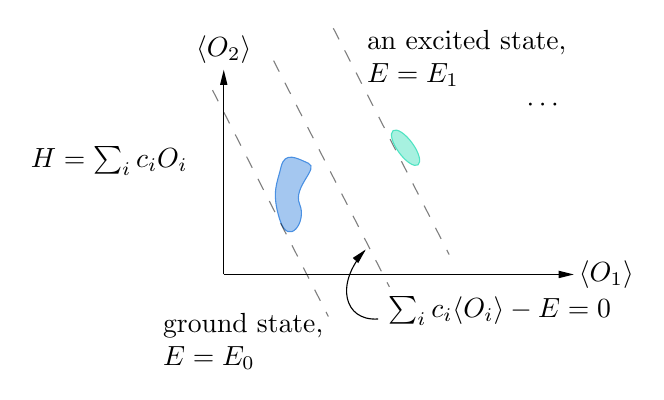
\begin{tikzpicture}[x=0.75pt,y=0.75pt,yscale=-0.6,xscale=0.6]
%uncomment if require: \path (0,353); %set diagram left start at 0, and has height of 353

%Straight Lines [id:da904255078328454] 
\draw    (177,246) -- (456,246) ;
\draw [shift={(458,246)}, rotate = 180] [fill={rgb, 255:red, 0; green, 0; blue, 0 }  ][line width=0.08]  [draw opacity=0] (12,-3) -- (0,0) -- (12,3) -- cycle    ;
%Straight Lines [id:da28860077544833507] 
\draw    (177,246) -- (177,83.73) ;
\draw [shift={(177,81.73)}, rotate = 90] [fill={rgb, 255:red, 0; green, 0; blue, 0 }  ][line width=0.08]  [draw opacity=0] (12,-3) -- (0,0) -- (12,3) -- cycle    ;
%Shape: Polygon Curved [id:ds05129166801576668] 
\draw  [color={rgb, 255:red, 74; green, 144; blue, 226 }  ,draw opacity=1 ][fill={rgb, 255:red, 74; green, 144; blue, 226 }  ,fill opacity=0.5 ] (223,159.73) .. controls (226,146.73) and (236,152.73) .. (245,156.73) .. controls (254,160.73) and (232,175.73) .. (238,189.73) .. controls (244,203.73) and (229,224.27) .. (222,202) .. controls (215,179.73) and (220,172.73) .. (223,159.73) -- cycle ;
%Straight Lines [id:da6483527344854445] 
\draw [color={rgb, 255:red, 0; green, 0; blue, 0 }  ,draw opacity=0.5 ] [dash pattern={on 4.5pt off 4.5pt}]  (168,98) -- (261,279.73) ;
%Straight Lines [id:da0036541181567224523] 
\draw [color={rgb, 255:red, 0; green, 0; blue, 0 }  ,draw opacity=0.5 ] [dash pattern={on 4.5pt off 4.5pt}]  (217,74.27) -- (310,256) ;
%Straight Lines [id:da34767057063343554] 
\draw [color={rgb, 255:red, 0; green, 0; blue, 0 }  ,draw opacity=0.5 ] [dash pattern={on 4.5pt off 4.5pt}]  (265,48.27) -- (358,230) ;
%Shape: Ellipse [id:dp302165402812995] 
\draw  [color={rgb, 255:red, 80; green, 227; blue, 194 }  ,draw opacity=1 ][fill={rgb, 255:red, 80; green, 227; blue, 194 }  ,fill opacity=0.5 ] (312.97,130.5) .. controls (310.07,132.62) and (312.21,140.48) .. (317.75,148.06) .. controls (323.29,155.64) and (330.13,160.08) .. (333.03,157.96) .. controls (335.93,155.84) and (333.79,147.98) .. (328.25,140.4) .. controls (322.71,132.81) and (315.87,128.38) .. (312.97,130.5) -- cycle ;
%Curve Lines [id:da7414078371933952] 
\draw    (301,281.73) .. controls (273.42,283.7) and (266.21,253.65) .. (289.9,227.21) ;
\draw [shift={(291,226)}, rotate = 133.09] [fill={rgb, 255:red, 0; green, 0; blue, 0 }  ][line width=0.08]  [draw opacity=0] (12,-3) -- (0,0) -- (12,3) -- cycle    ;

% Text Node
\draw (460,246) node [anchor=west] [inner sep=0.75pt]    {$\langle O_{1} \rangle $};
% Text Node
\draw (177,78.33) node [anchor=south] [inner sep=0.75pt]    {$\langle O_{2} \rangle $};
% Text Node
\draw (307,261.4) node [anchor=north west][inner sep=0.75pt]    {$\sum _{i} c_{i} \langle O_{i} \rangle -E=0$};
% Text Node
\draw (259,275) node [anchor=north east] [inner sep=0.75pt]   [align=left] {ground state,\\$\displaystyle E=E_{0}$};
% Text Node
\draw (290,97.27) node [anchor=south west] [inner sep=0.75pt]   [align=left] {an excited state,\\$\displaystyle E=E_{1}$};
% Text Node
\draw (418,103.4) node [anchor=north west][inner sep=0.75pt]    {$\cdots $};
% Text Node
\draw (20,141.4) node [anchor=north west][inner sep=0.75pt]    {$H=\sum _{i} c_{i} O_{i}$};


\end{tikzpicture}

\end{center}

\end{frame}

\begin{frame}
\frametitle{Bootstrap for generic systems}

\textbf{The procedure of numerical bootstrap}   

Input data:
\begin{itemize}
    \item Determine $N$ operators $\{O_i\}$ as the basis of all operators.
    Example: normal ordered, with a length cutoff 
    \item Data of equality constraints: Hamiltonian, symmetry, etc.
    \item Commutation rules, normal ordering rules, etc. so that $O_i O_j$ can be expanded in terms of $\{O_i\}$
    \item Hamiltonian $H = \sum_i c_i O_i$
\end{itemize}

Building the optimization problem:
\begin{enumerate}
    \item Declare $N$ variables $\{X_i\}$, $X_i = \expval*{O_i}$ after optimization
    \item Impose equality constraints on $\{X_i\}$ according to e.g. $\expval*{\comm{H}{O}} = 0$ 
    \item Imposing semidefinite constraint on $M_{ij} = \expval*{O_i^\dagger O_j}$, so that after optimization $\expval*{O^\dagger O} \geq 0$ for every $O$
    \item Optimize $\sum_i c_i X_i$
\end{enumerate}

\end{frame}

\begin{frame}
\frametitle{Bootstrap for generic systems}

\textbf{Why we need numerical bootstrap}

\begin{itemize}
    \item Because it doesn't fail with strong non-perturbative effects.\footnote{\href{https://arxiv.org/abs/2108.11416}{arXiv 2108.11416}}
    \item Because if done correctly, it gives the \emph{lower} bound of ground state energy
    \begin{itemize}
        \item Density matrix = linear functional $\mathcal{F}$ from operators to numbers
        \item Predicted $E_0$ = $\min_{\mathcal{F} \text{constrained}} \mathcal{F}[H]$
        \item Real ground state also constrained $\Rightarrow$ real $E_0 > $ predicted $E_0$
    \end{itemize}
\end{itemize}    

\end{frame}

\begin{frame}
\frametitle{Bootstrap for generic systems}

\textbf{Some technical aspects of the problem}

When building the optimization problem: 
\begin{itemize}
    \item A little symbolic calculation required
    \item Auto normal ordering of $O_i O_j$ given the operator algebra
    \item Auto commutator: $\comm{A}{B}$ = normal ordered $AB$ - normal ordered $BA$ 
\end{itemize}

\end{frame}

\begin{frame}
\frametitle{Bootstrap for generic systems}

For optimization itself
\begin{itemize}
    \item \concept{Linear semidefinite programming (linear SDP)} when using $\expval*{\comm{H}{O}} = 0$
    ($\expval{HO}$ and $\expval*{OH}$ being linear combination of $\{O_i\}$)
    \begin{itemize}
        \item Convex optimization\footnote{See \href{https://en.wikipedia.org/wiki/Semidefinite_programming}{Wikipedia}} 
        \item Mature solvers like SCS\footnote{\href{https://github.com/cvxgrp/scs}{https://github.com/cvxgrp/scs}} or CSDP\footnote{\href{https://github.com/coin-or/Csdp}{https://github.com/coin-or/Csdp}}
    \end{itemize}
    \item \concept{Nonlinear semidefinite programming (nonlinear SDP)} when using $\expval*{{H}{O}} = E \expval*{O}$
    because there are optimization variables in $E$
    \begin{itemize}
        \item No solver mature enough\footnote{See the discussion before Sec.~1.1 in \href{https://arxiv.org/abs/2108.04830}{arXiv 2108.04830}. Also, no solver supporting both SDP and nonlinear programming (NLP) is listed in \href{https://jump.dev/JuMP.jl/stable/installation/}{the solver list of JuMP.jl}.}
    \end{itemize}
\end{itemize}    

\end{frame}

\begin{frame}
\frametitle{Bootstrap for generic systems}

\begin{itemize}
    \item linear SDP (constraints: $\expval*{\comm{O}{H}} = 0$, thermal states allowed) easy
    \item nonlinear SDP (constraints: $\expval*{{O}{H}} = E \expval{O}$, no thermal states) hard 
\end{itemize}

\textbf{Example of linear SDP (and why it's easy)} 

\begin{columns}
    \begin{column}{0.5\textwidth}
        \[
            \begin{aligned}
                \max\  &M_{11} + 2 M_{12}, \ \text{s.t.} \\
                &M = M^\top, \ M \geq 0, \\
                &M_{11} + M_{12} + M_{13} = - 0.5, \\
                &M_{22} = 2 M_{11} + 3 M_{12} + 1, \\
                &M_{23} + 4 M_{11} = 0, \\
                &M_{33} = 4 M_{11} + 5M_{12}.
            \end{aligned}
        \]
        \begin{itemize}
            \item Convex feasible domain
            \item Linear objective $\Rightarrow$ minimum at the edge
        \end{itemize}
    \end{column}
    \begin{column}{0.5\textwidth}
        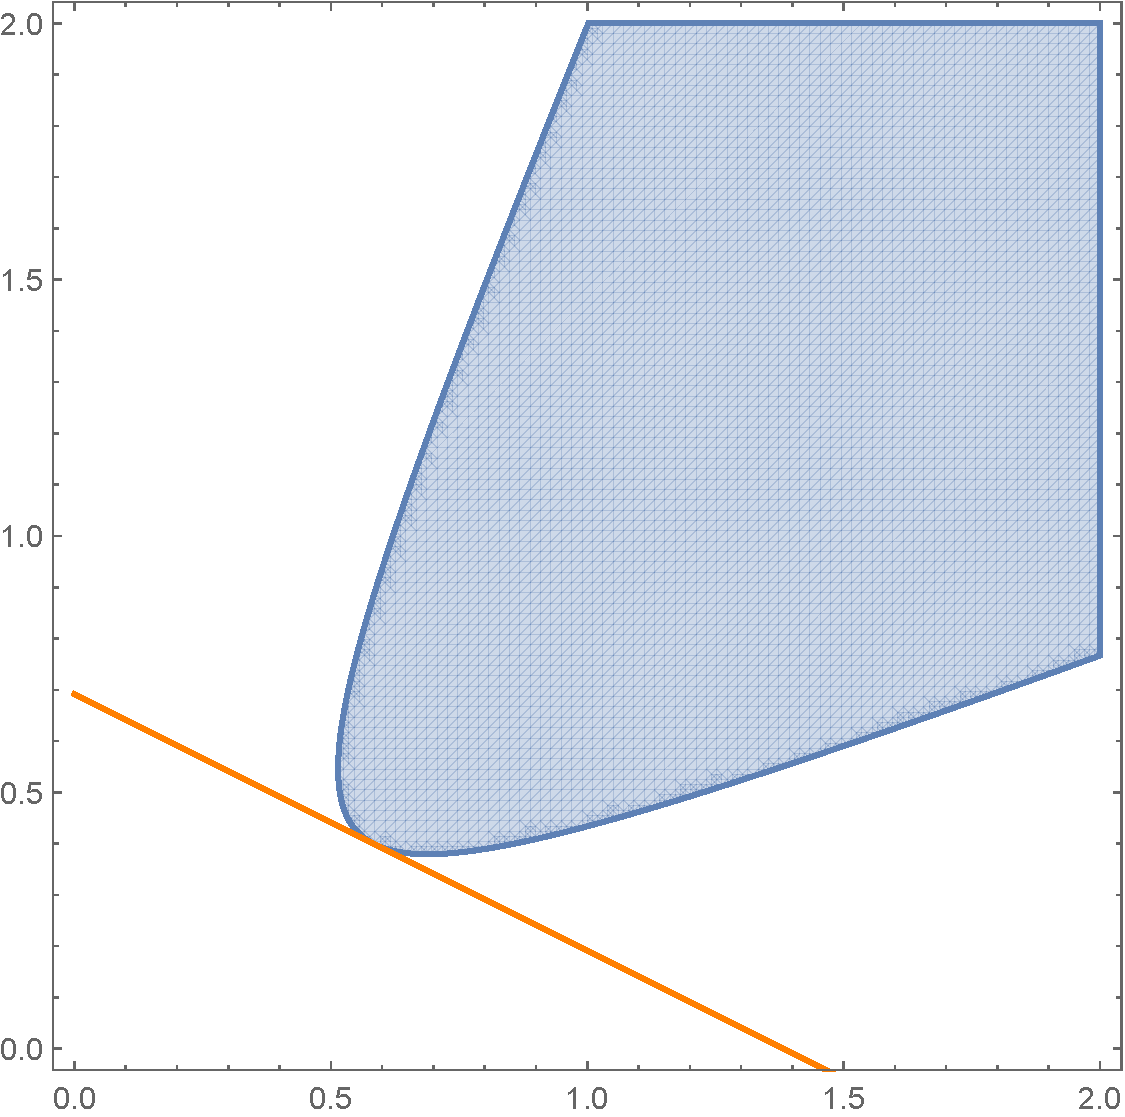
\includegraphics[width=\textwidth]{jump-toy-2-benchmark-feasible-domain-and-result.pdf}
    \end{column}
\end{columns}

\end{frame}

\begin{frame}
\frametitle{Example: $x^4$ anharmonic oscillator}

Consider the anharmonic oscillator\footnote{The example is provided in \href{https://arxiv.org/abs/2004.10212}{arXiv 2004.10212}}, a famous failure of perturbation theory\footnote{Carl M. Bender and Tai Tsun Wu, Anharmonic Oscillator. Phys. Rev. 184, 1231.}
\begin{equation}
    H = x^2 + p^2 + g x^4.
\end{equation}

\begin{itemize}
    \item Symmetry: $x \to -x$ $\Rightarrow$ $\expval*{x^n} = 0$ with odd $n$
    \item Deriving equality constraints:
    \begin{itemize}
        \item $\mathcal{O}=x^{s}$ and $\mathcal{O}=x^{t} p$ in $\langle[H, \mathcal{O}]\rangle=0$ 
        \item $\mathcal{O}=x^{t-1}$ in $\langle\mathcal{O} H\rangle=E\langle\mathcal{O}\rangle$
    \end{itemize}
    \item So finally we have
        \begin{equation}
            \begin{aligned}
                &E=2\left\langle x^{2}\right\rangle+3 g\left\langle x^{4}\right\rangle, \\
                &4 t E\left\langle x^{t-1}\right\rangle +t(t-1)(t-2)\left\langle x^{t-3}\right\rangle -4(t+1)\left\langle x^{t+1}\right\rangle \\
                &\quad -4 g(t+2)\left\langle x^{t+3}\right\rangle=0 
            \end{aligned}
        \end{equation}
    \item Only independent variables: $\expval{x^2}$ and $E$, so nonlinear SDP is possible
    \item SDP constraint: $M_{ij} = \expval*{x^{i+j}}, M \geq 0$
\end{itemize}

\end{frame}

\begin{frame}[fragile]
\frametitle{Example: $x^4$ anharmonic oscillator}

\begin{itemize}
    \item Reproduce Fig.~1 in \href{https://arxiv.org/abs/2004.10212}{arXiv 2004.10212} by brutal force searching
    \item Numerical bootstrap can be quite precise! (high resolution Mathematica plotting required to find the allowed region)
\end{itemize}

\begin{columns}
    
    \begin{column}{0.5\textwidth}
        \lstset{language=Mathematica, basicstyle=\tiny, xleftmargin=-40pt}
        % Code from oscillator-simple-prototype\2022-1-20.nb
        \begin{lstlisting}
            expectedX[0] := 1;
            expectedX[2] := x2;
            expectedX[4] := 1/(3 g) (E0 - 2 x2);
            expectedX[u_?EvenQ] := 
            1 / (4 g ((-3 + u) + 2)) * 
            (4 (-3 + u) E0 expectedX[(-3 + u) - 1] 
            + (-3 + u) ((-3 + u) - 1) ((-3 + u) - 2) 
                expectedX[(-3 + u) - 3] 
            - 4 ((-3 + u) + 1) expectedX[(-3 + u) + 1]);

            matPositive[K_] := 
            Table[expectedX[i+j], {i, 0, K}, {j, 0, K}];

            RegionPlot[
            AllTrue[Eigenvalues[matPositive[9] /. g -> 1], 
                # >= 0 &], 
            {E0, 1.35, 1.44}, {x2, 0.294, 0.311}, 
            PlotPoints -> 100]
        \end{lstlisting}
    \end{column}

    \begin{column}{0.5\textwidth}
        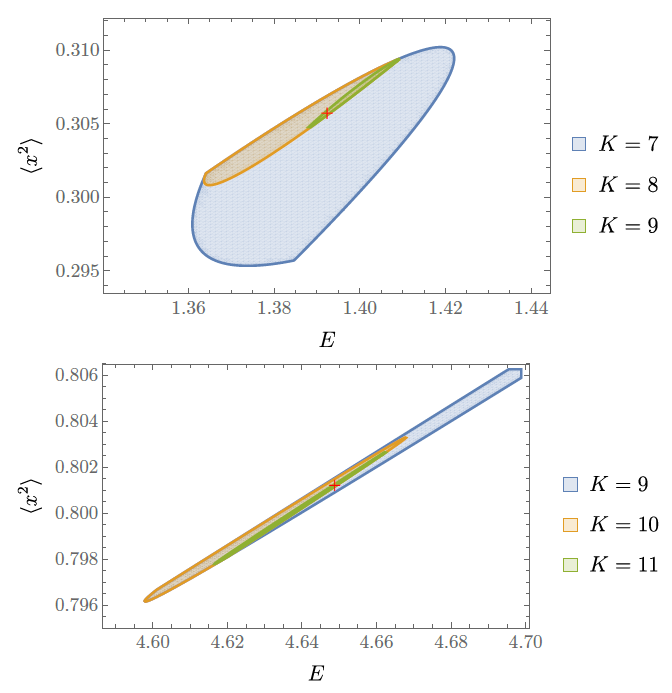
\includegraphics[width=\textwidth]{oscillator-bootstrap-feasible-domains.PNG}
    \end{column}
\end{columns} 

\end{frame}

\begin{frame}
\frametitle{Example: $x^4$ anharmonic oscillator}

\textbf{Benchmark}

\begin{itemize}
    % program: oscillator-simple-prototype\stationary-schrodinger.jl
    \item Solving the Schr\"{o}dinger equation with finite difference method with $\Delta x = 0.05$: $E_0 = 1.3919$
    % program: oscillator-simple-prototype\2022-1-20.nb
    \item Numerical bootstrap with $K=11$: $E_0 = 1.3922$
\end{itemize}  

\end{frame}

\begin{frame}
\frametitle{More examples}

\textbf{Double-well potential}\footnote{See \href{https://arxiv.org/abs/2108.11416}{arXiv 2108.11416}}

\begin{columns}
    \begin{column}{0.5\textwidth}
        \begin{itemize}
            \item Another famous non-perturbative model (instantons between the wells)
            \item \begin{equation}
                H=p^{2}-m^{2} x^{2}+g x^{4}+\mathcal{V}_{0}
            \end{equation}
            \item Error between predicted split between the ground state and the first excited state and the dilute instanton approximation goes down as the two wells are separated.
        \end{itemize}
    \end{column}
    \begin{column}{0.5\textwidth}
        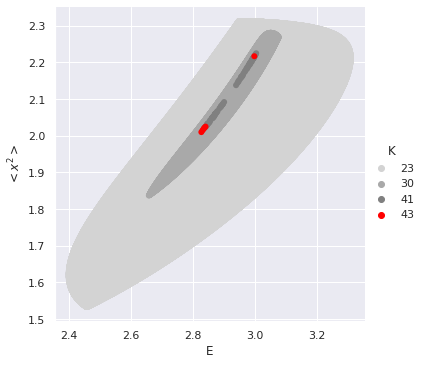
\includegraphics[width=\textwidth]{double-well-bootstrap-feasible-domain.png}
    \end{column}
\end{columns}

\end{frame}

\begin{frame}
\frametitle{More examples}

\textbf{Matrix model}\footnote{See \href{https://arxiv.org/pdf/2108.04830.pdf}{arXiv 2108.04830} and \href{https://arxiv.org/abs/2004.10212}{arXiv 2004.10212}}

\begin{itemize}
    \item Impossible to solve otherwise
    \item A specific case associated with $M$-theory\footnote{\href{https://arxiv.org/abs/hep-th/9610043}{arXiv hep-th 9610043}}
    \item (Inherent) nonlinear constraints
    \begin{itemize}
        \item Relaxed bootstrap in Sec.~4 in \href{https://arxiv.org/pdf/2108.04830.pdf}{arXiv 2108.04830}
        \item trust-region sequential SDP in \href{https://github.com/hanxzh94/matrix-bootstrap}{Xizhi Han's code}
    \end{itemize}
\end{itemize}

\end{frame}

\begin{frame}
\frametitle{More examples}

\textbf{Hubbard model}\footnote{See \href{https://arxiv.org/abs/2006.06002}{2006.06002}.}

Bootstrapping of models in condensed matter physics -- No sign problem!

\[
    \begin{array}{||c|c|c|c|c||}
        \hline n=1 & U=2 & U=4 & U=6 & U=8 \\
        \hline\left.E_{\mathrm{lb}}\right|_{K=7} & -1.221 & -0.913 & -0.705 & -0.565 \\
        \left.E_{\mathrm{lb}}\right|_{K=\infty} & - & - & -0.66(2) & -0.54(2) \\
        E_{\mathrm{AFQMC}} & -1.1763(2) & -0.8603(2) & -0.6568(3) & -0.5247(2) \\
        E_{\mathrm{DMET}} & -1.1764(3) & -0.8604(3) & -0.6562(5) & -0.5234(10) \\
        E_{\mathrm{DMRG}} & -1.176(1) & -0.8605(5) & -0.6565(1) & -0.5241(1) \\
        \hline n=0.875 & U=2 & U=4 & U=6 & U=8 \\
        \hline\left.E_{\mathrm{lb}}\right|_{K=7} & -1.316 & -1.103 & -0.963 & -0.867 \\
        \left.E_{\mathrm{lb}}\right|_{K=\infty} & - & - & -0.86(5) & -0.77(3) \\
        E_{\mathrm{DMET}} & -1.2721(6) & -1.031(3) & -0.863(13) & -0.749(7) \\
        \hline
        \end{array}
\]

\begin{itemize}
    \item Operator space cutoff: $l(c_{x_1 \sigma_1}^{(\dagger)}) = r + \sum_{i=1}^r \|x_i \|_1 \leq K$ 
    \item Ground state energy lower bounded
\end{itemize}

\end{frame}

\begin{frame}
\frametitle{Discussion}

\textbf{What can be immediately done}

\begin{itemize}
    \item Bootstrapping anharmonic oscillator by linear SDP
    \item Reproduce the results of Hubbard model 
\end{itemize}

\textbf{Future perspectives}

\begin{itemize}
    \item Bootstrapping a \emph{class} of models (e.g. ``all possible models made by $x$ and $p$'')
    \begin{itemize}
        \item Extending what is done in conformal bootstrap (e.g. ``all possible CFTs made by $\sigma$ and $\epsilon$'') to all kind of models
    \end{itemize}
    \item Extracting thermal information from $\expval*{\comm{O}{H}} = 0$ bootstraps
    \item What constraints are effective? 
    \begin{itemize}
        \item Can wave function ansatz (e.g. DMRG) provide some hints?
    \end{itemize}
\end{itemize}

\end{frame}

\end{document}